% -*- root: ../assignment.tex -*-
\subsection*{Linear Dynamics Systems -- State space view}
\begin{enumerate}[resume]
    \item Derive the state and measurement equations for the following composite systems, assuming the system $H_i$ to have the parameters $\ct{\mf{A}_i, \mf{B}_i, \mf{C}_i, \mf{D}_i}$.
    \begin{center}
        \begin{tikzpicture}[scale=0.75, transform shape, thick, node distance=2cm]
        \draw
            node [input, name=input1] {} 
            node [block, right of=input1] (sys1) {{\large $H_1$}}
            node [block, right of=sys1] (sys2) {{\large $H_2$}}
            node [input, right of=sys2, name=output1] {};
            \draw[-latex] node [above] {{\large $\mf{u}\ct{t}$}} (input1) -- node {} (sys1);
            \draw[-latex](sys1) -- node {} (sys2);
            \draw[-latex](sys2) -- node[above] {\large $\mf{y}\ct{t}$} (output1);
            \node[]  at (-1,0) {\textbf{(a)}};
        \end{tikzpicture}

        \begin{tikzpicture}[scale=0.75, transform shape, thick, node distance=2cm]
        \draw
            node [input, name=input1] {}
            node [input, right of=input1, name=tempin1] {} 
            node [input, below of=tempin1, name=tempin2] {} 
            node [block, right of=tempin1] (sys1) {{\large $H_1$}}
            node [block, right of=tempin2] (sys2) {{\large $H_2$}}
            node [sum, right of=sys1] (suma1) {$\suma$} 
            node [input, right of=sys2, name=tempout2] {}
            node [input, right of=suma1, name=output1] {};

            \draw[-] node [above] {{\large $\mf{u}\ct{t}$}} (input1) -- node {} (tempin1);
            \draw[-latex] node {} (tempin1) -- node {} (sys1);
            \draw[-] node {} (tempin1) -- node {} (tempin2);
            \draw[-latex] node {} (tempin2) -- node {} (sys2);
            \draw[-latex](sys1) -- (suma1);
            \draw[-] node {} (sys2) -- node {} (tempout2);
            \draw[-latex] node {} (tempout2) -- node {} (suma1);
            \draw[-latex] node {} (suma1) -- node[above] {\large $\mf{y}\ct{t}$} (output1);
            \node[]  at (-1,0) {\textbf{(b)}};
        \end{tikzpicture}

        \begin{tikzpicture}[scale=0.75, transform shape, thick, node distance=2cm]
        \draw
            node [input, name=input1] {}
            node [sum, right of=input1] (suma1) {$\suma$} 
            node [input, below of=suma1, name=tempfb] {} 
            node [block, right of=suma1] (sys1) {{\large $H_1$}}
            node [input, right of=sys1, name=tempout1] {}
            node [input, right of=tempout1, name=output1] {}
            node [input, below of=tempout1, name=tempout2] {}
            node [block, below of=sys1] (sys2) {{\large $H_2$}};

            \draw[-latex] node [above] {{\large $\mf{u}\ct{t}$}} (input1) -- node {} (suma1);
            \draw[-latex] node {} (suma1) -- node {} (sys1);
            \draw[-] node {} (sys1) -- node {} (tempout1);
            \draw[-latex] node {} (tempout1) -- node {} (output1);
            \draw[-] node {} (tempout1) -- node {} (tempout2);
            \draw[-latex] node {} (tempout2) -- node {} (sys2);
            \draw[-] node {} (sys2) -- node {} (tempin2);
            \draw[-latex] node {} (tempin2) -- node {} (suma1);
            \draw[-latex] node {} (tempout1) -- node[above] {\large $\mf{y}\ct{t}$} (output1);
            \node[]  at (-1,0) {\textbf{(c)}};
        \end{tikzpicture}
    \end{center}
    
    \item Derive the state and measurement equation for the following system, where the input is the force $f$ applied to mass $m_2$, and the output is the acceleration of the mass $m_1$ and velocity of mass $m_2$.
    \begin{center}
    \begin{tikzpicture}[every node/.style={draw,outer sep=0pt,thick}, scale=0.8]
    %define the spring
    \tikzstyle{spring}=[thick,decorate,decoration={zigzag,pre length=0.12cm,post length=0.12cm,amplitude=1.3mm,segment length=6}]

    %define the dashpot
    \tikzstyle{damper}=[thick,decoration={markings,
      mark connection node=dmp,
      mark=at position 0.5 with 
      {
          \node (dmp) [thick,inner sep=0pt,transform shape,rotate=-90,minimum width=15pt,minimum height=3pt,draw=none] {};    
          \draw [thick] ($(dmp.north east)+(2pt,0)$) -- (dmp.south east) -- (dmp.south west) -- ($(dmp.north west)+(2pt,0)$);
          \draw [thick] ($(dmp.north)+(0,-5pt)$) -- ($(dmp.north)+(0,5pt)$);
      }
    }, decorate]

    %define the spring-dashpot
    \tikzstyle{spr-dash}=[thick,decorate,decoration={markings,
      mark connection node=sqr,
      mark=at position 0.5 with
      {
          \node (sqr) [thick,minimum width=16pt,minimum height=24pt,draw=none] {};
          \draw [thick] (sqr.north west) -- (sqr.north east);
          \draw [thick] (sqr.south west) -- (sqr.south east);
          \draw [spring] (sqr.south west) -- (sqr.north west);
          \draw [damper] (sqr.south east) -- (sqr.north east);
      }
      }]

    %define the ground
    \tikzstyle{ground}=[fill,pattern=north east lines,draw=none,minimum width=0.75cm,minimum height=0.3cm]

    \begin{scope}[xshift=5.5cm]
    %draw the frame mass
    \node (M1) [minimum width=1cm,minimum height=1cm] {$m_1$};
     
    %draw the vehicle mass
    \node (M2) at (M1.north) [yshift=+1.8cm, minimum width=1cm, minimum height=1cm] {$m_2$};

    \node (ground-medium) at (M1.south) [ground,yshift=-1.3cm,minimum width=4cm,anchor=north] {};
    \draw (ground-medium.north west) -- (ground-medium.north east);

    \draw [spr-dash] (ground-medium.north) -- (M1.south);
    \node [draw=none] at ($(ground-medium.north)+(-1cm,0.7cm)$) {$k_{1}$};
    \node [draw=none] at ($(ground-medium.north)+(1.1cm,0.7cm)$) {$b_{1}$};
    \draw [spr-dash] (M1.north) -- (M2.south);
    \node [draw=none] at ($(M1.north)+(-1.0cm,0.7cm)$) {$k_{2}$};
    \node [draw=none] at ($(M1.north)+(1.1cm,0.7cm)$) {$b_{2}$};
     
    \draw [-latex,thick] (M2.north) ++ (0, 0.5cm) -- (M2.north);
    \draw [dashed,thin] (M2.east) ++ (0.5cm, 0) -- +(1.0cm, 0);
    \node [draw=none, right] at ($(M2.east) + (1.5cm, 0)$) {$x_{2}$};

    \draw [dashed,thin] (M1.west) ++ (-0.5cm, 0) -- +(-1.0cm, 0);
    \node [draw=none, left] at ($(M1.west) + (-1.5cm, 0cm)$) {$x_{1}$};

    \node [draw=none, yshift=0.7cm] at (M2.north) {$f$};
    \end{scope}
    \end{tikzpicture}
    \end{center}

    Assume now that instead of $f$ the input to this was the position of the mass $m_2$ (i.e. $x_2$) and the output of interest was the acceleration of the mass $m_1$. What would be correspondoing state and measurement equations in this case?

    \item Obtain a state space representation for the following systems:
    \begin{enumerate}
        \item $\sum_{i=0}^n a_iy^{\ct{i}} = \sum_{j=0}^m b_jx^{\ct{j}}$, where $x^{\ct{k}} = \frac{d^k}{dt^k}x\ct{t}$
        \item $\sum_{i=0}^n a_iy\dt{k+i} = \sum_{j=0}^m b_jx\dt{k+j}$
    \end{enumerate}

    \item Write down the state and measurement equations for the following system with the scalar input $u\dt{k}$ and output $\mf{y}\dt{k} = \bmx y_1\dt{k}\\ y_2\dt{k}\emx$. 

    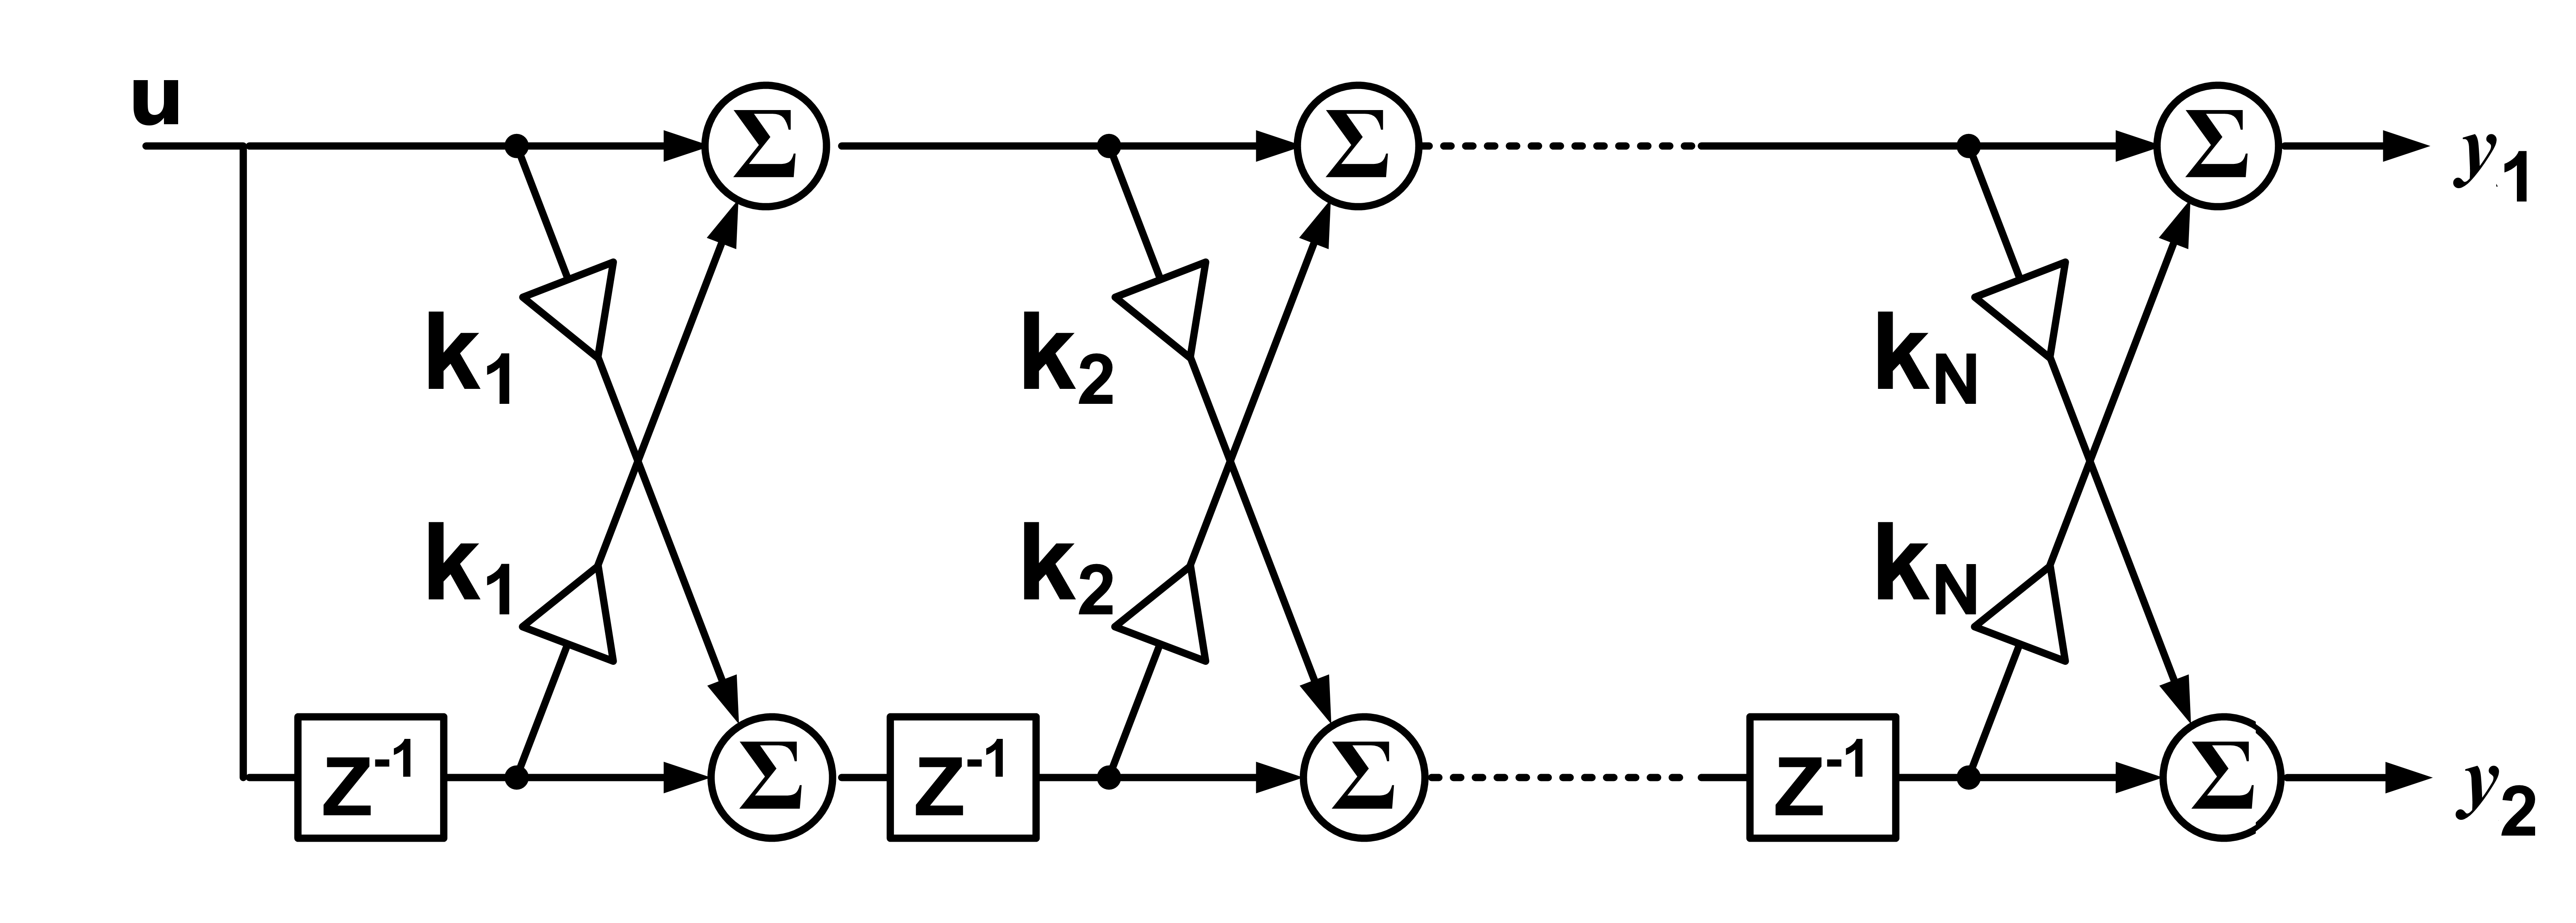
\includegraphics[width=0.45\textwidth]{sections/figs/latticefilt.png}

    \item The following model shows two media and their constituent elements. Medium 1 consists of elements with mass $M_1$ which are interconnected through a spring and damper in parallel with spring constant $k_1$ and damping coefficient $b_1$. Medium 2 consits of elements with mass $M_2$ connected through $k_2$ and $b_2$. At the interface $M_1$ and $M_2$ are connected through $k_3$ nd $b_3$.

    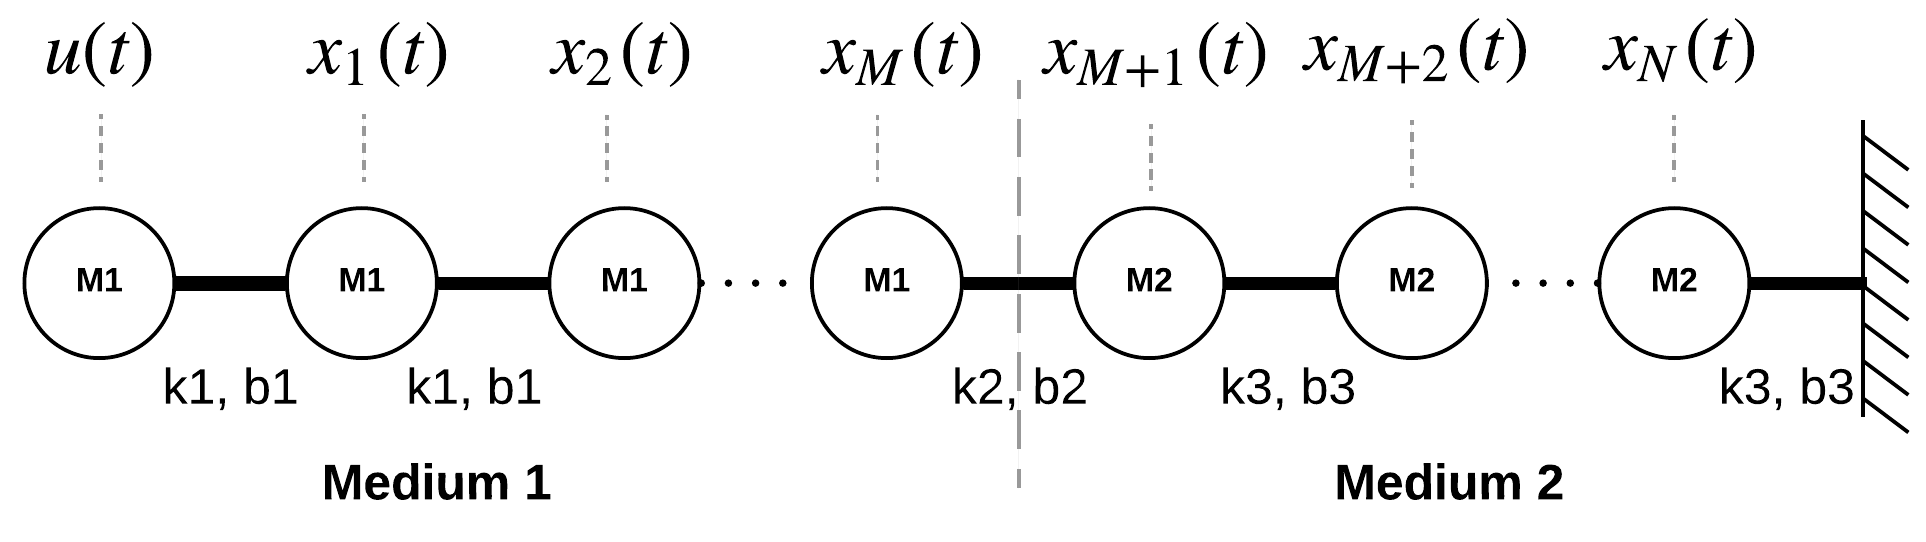
\includegraphics[width=0.45\textwidth]{sections/figs/wavetx.png}    

    The input to this system is $u\ct{t}$ which is the position imposed on the let most element in medium 1. The output of the system are the successive differences in the positions of the massess.
    \[ y_i\ct{t} = x_{i+2}\ct{t} - x_{i+1}\ct{t} \, ,\,\,\, 1 \leq i \leq N-2 \]

    Derive the state and measurement equations for the system.


\end{enumerate}
% \vfill